\documentclass[12pt,a4paper]{article}
\usepackage[utf8]{inputenc}
\usepackage[spanish]{babel}
\usepackage{graphicx}
\usepackage{hyperref}
\usepackage{geometry}
\usepackage{fancyhdr}
\usepackage{titlesec}
\usepackage{booktabs}
\usepackage{longtable}
\usepackage{xcolor}
\usepackage{listings}
\usepackage{enumitem}
\usepackage{float}
\usepackage{graphicx}
\usepackage{tikz}
\usetikzlibrary{calc}
\usepackage{array,booktabs,longtable}
\newcolumntype{P}[1]{>{\raggedright\arraybackslash}p{#1}}

\geometry{left=2.5cm,right=2.5cm,top=2.5cm,bottom=2.5cm}

% Configuración de hipervínculos
\hypersetup{
    colorlinks=true,
    linkcolor=blue,
    filecolor=magenta,      
    urlcolor=cyan,
    pdftitle={UI2Code - Sistema Multi-Agente},
    pdfauthor={Qualindi, Denardi, Valdez, Masoller},
}

% Configuración de código
\lstset{
    basicstyle=\ttfamily\small,
    breaklines=true,
    frame=single,
    xleftmargin=0.5cm,
    xrightmargin=0.5cm
}

% Encabezado y pie de página
\pagestyle{fancy}
\fancyhf{}
\rhead{UI2Code - Sistema Multi-Agente}
\lhead{PLN III - FIUBA}
\cfoot{\thepage}

\begin{document}

% Portada
\begin{titlepage}
    \centering

    % ===== Cabecera con imagen =====
    % Reemplazá por la ruta y tamaño que quieras
    
\includegraphics[width=0.6\textwidth]{./docs/uba.png}\\[1cm]
    
    {\LARGE\bfseries TRABAJO PRÁCTICO FINAL\\[0.5cm]}
    {\Large PROCESAMIENTO DEL LENGUAJE NATURAL III\\[0.3cm]}
    {\large MAESTRÍA EN INTELIGENCIA ARTIFICIAL\\[0.2cm]}
    {\large Universidad de Buenos Aires (FIUBA)\\[1cm]}
    
    \rule{\textwidth}{1.5pt}\\[0.4cm]
    {\Huge\bfseries UI2Code\\[0.2cm]}
    {\LARGE Sistema Multi-Agente para conversión\\[0.1cm] de diseños UI a código HTML/Tailwind CSS y prompt a código\\[0.2cm]}
    \rule{\textwidth}{1pt}\\[1cm]
    
    {\large\bfseries Equipo:\\[0.3cm]}
    \begin{tabular}{ll}
        Noelia Melina Qualindi & \texttt{noelia.qualindi@gmail.com} \\
        Fabricio Denardi & \texttt{denardifabricio@gmail.com} \\
        Jorge Ceferino Valdez & \texttt{jorgecvaldez@gmail.com} \\
        Bruno Masoller & \texttt{brunomaso1@gmail.com}
    \end{tabular}\\[1cm]
    
    {\large\bfseries Docentes:\\[0.3cm]}
    Oksana Bokhonok, Abraham Rodríguez\\[1cm]
    
    \begin{tikzpicture}[remember picture, overlay]
      \node[
        anchor=south east,
        xshift=0.5cm,   % + hacia afuera (derecha). Probá 0.2–0.8cm
        yshift=-0.5cm   % - hacia afuera (abajo).  Probá -0.2 a -0.8cm
      ] at (current page.south east)
      {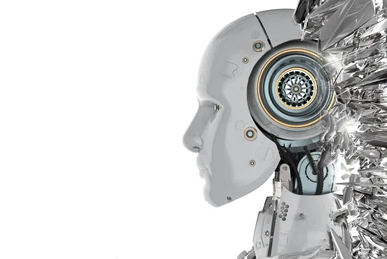
\includegraphics[width=0.40\paperwidth, trim=0 0 0 0, clip]{./docs/robot.png}};
    \end{tikzpicture}
        {\large Repositorio del proyecto:\\[0.2cm]}
        \url{https://github.com/jorgeceferinovaldez/ui2code-rag}\\[0.5cm]
            {\small \today}

% --------------------------------------------------------

\end{titlepage}

\tableofcontents
\newpage

\section{Resumen}

UI2Code-RAG es un sistema multi-agente que convierte diseños de interfaz de usuario (imágenes estáticas) en código HTML + Tailwind CSS funcional y estandarizado, combinando análisis visual con Inteligencia Artificial y RAG híbrido (BM25 + embeddings vectoriales + re-ranking con cross-encoder) sobre un corpus de 900 ejemplos HTML/CSS del dataset WebSight.

La arquitectura se orquesta mediante un \textbf{Orchestrator Agent A2A} que coordina tres agentes especializados:
\begin{itemize}
    \item \textbf{Visual Agent}: Análisis multimodal de imágenes UI
    \item \textbf{RAG Agent}: Búsqueda híbrida de patrones de código similares
    \item \textbf{Code Agent}: Generación de código HTML/Tailwind con validación anti-hallucination
\end{itemize}

El sistema incluye guardrails de validación de salidas (JSON, HTML, web sanitization) y una aplicación Streamlit multipágina que proporciona interfaces para: UI-to-Code, Query Interface, Evaluaciones, System Status y Corpus Information.

\section{Presentación del Problema}

En ingeniería de software, uno de los principales problemas para las empresas que desarrollan grandes sistemas de información es el balance entre \textbf{estándares flexibles y estándares forzosos}. La estandarización de las prácticas de ingeniería de software siempre es mejor, usualmente sin importar el caso de uso, pero esto lleva a un mayor ``lead time''. En un mundo actual donde el ``time to market'' es uno de los principales atributos dentro de un proceso, este complejo problema lleva a soluciones del tipo \textit{``convention over configuration''}. 

El potencial de los LLMs (Large Language Models) los hace aptos para este tipo de desarrollo, donde se puede forzar la convención de forma transparente para el desarrollador.

\subsection{Contexto y Motivación}

Con este tema en mente, \textbf{UI2Code} se posiciona con la misión de brindar a los desarrolladores \textbf{estandarización automática}, al generar código que cumpla con los estándares de la empresa en base a un diseño preliminar. Por un lado, los desarrolladores pueden partir de una base estandarizada y, por el otro, se reducen los tiempos de desarrollo para las empresas.

\subsection{Desafíos Identificados}

Sin embargo, existen varios desafíos técnicos:

\begin{enumerate}
    \item \textbf{Alucinación de modelos}: Los modelos de visión-lenguaje (VLMs) y LLMs pueden alucinar estructura o estilos inexistentes cuando deben generar código a partir de una sola imagen.
    
    \item \textbf{Ambigüedad semántica}: Distintas UIs presentan ambigüedad en layout, jerarquías, tipografías y breakpoints responsivos.
    
    \item \textbf{Falta de evidencia explícita}: Ciertos componentes no tienen evidencia clara en la imagen para inferir su implementación técnica.
    
    \item \textbf{Necesidad de contexto reutilizable}: Se requiere un corpus de patrones de código que guíe la generación y mantenga la consistencia.
    
    \item \textbf{Verificación de formato}: Es necesario implementar validaciones para reducir alucinaciones y obtener código realmente utilizable.
\end{enumerate}

\section{Objetivos}

\subsection{Objetivo General}

Desarrollar un sistema multi-agente que convierta imágenes de interfaces de usuario en código HTML/Tailwind CSS ``listo para usar'', minimizando alucinaciones y maximizando la reutilización de patrones estandarizados.

\subsection{Objetivos Específicos}

\begin{itemize}[leftmargin=*]
    \item \textbf{Conversión UI-to-Code}: Transformar imágenes de diseños UI en código HTML/Tailwind funcional y estandarizado.
    
    \item \textbf{Recuperación y reutilización de patrones}: Implementar un sistema RAG híbrido para recuperar y reusar patrones de código similares, guiando la generación y reduciendo la deuda técnica.
    
    \item \textbf{Interfaz de usuario simplificada}: Exponer una interfaz web intuitiva para cargar imágenes, ajustar instrucciones personalizadas, visualizar resultados y descargar código generado.
    
    \item \textbf{Visibilidad del sistema}: Proporcionar dashboards de estado del sistema, métricas del corpus y health checks de los agentes.
    
    \item \textbf{Evaluación cuantitativa}: Implementar framework de evaluación con métricas estándar de recuperación de información.
\end{itemize}

\subsection{Alcance}

\begin{itemize}
    \item Inferencia mediante modelos de IA vía API (sin entrenamiento)
    \item Corpus curado de 900 patrones HTML/CSS del dataset WebSight
    \item Sistema RAG híbrido con BM25, búsqueda vectorial y re-ranking
    \item Validaciones de salida con Guardrails
    \item Arquitectura multi-agente con protocolo A2A (Agent-to-Agent)
\end{itemize}

\section{Técnicas y Tecnologías Utilizadas}

\subsection{Modelos de Inteligencia Artificial}

\subsubsection{Análisis Visual}
\begin{itemize}
    \item \textbf{Gemini 2.0 Flash Exp} (Google): Modelo de visión gratuito para análisis de layout, componentes y estilos
    \item \textbf{GPT-4 Vision} (OpenAI): Alternativa de pago con mayor precisión
    \item \textbf{Claude 3.5 Sonnet} (Anthropic): Opción premium para casos complejos
\end{itemize}

\subsubsection{Generación de Código}
\begin{itemize}
    \item \textbf{DeepSeek R1 Distill Llama 70B}: Modelo gratuito optimizado para código
    \item \textbf{DeepSeek R1}: Versión de pago con mejor calidad
    \item Acceso vía \textbf{OpenRouter}: Plataforma que unifica el acceso a múltiples modelos con precios competitivos
\end{itemize}

\subsection{Sistema RAG Híbrido}

El sistema implementa un pipeline de recuperación de información de tres capas:

\begin{enumerate}
    \item \textbf{Búsqueda léxica (BM25)}: Recuperación basada en términos exactos y frecuencia
    \item \textbf{Búsqueda vectorial (Semantic Search)}: 
    \begin{itemize}
        \item Embeddings con \texttt{sentence-transformers/all-MiniLM-L6-v2} (384 dimensiones)
        \item Almacenamiento en Pinecone Vector Database
        \item Namespace: \texttt{html-css-examples}
    \end{itemize}
    \item \textbf{Re-ranking con Cross-Encoder}:
    \begin{itemize}
        \item Modelo: \texttt{ms-marco-MiniLM-L-6-v2}
        \item Mejora la precisión del ranking final
    \end{itemize}
\end{enumerate}

\subsection{Infraestructura y Orquestación}

\subsubsection{Protocolo A2A (Agent-to-Agent)}
\begin{itemize}
    \item Comunicación basada en JSONRPC sobre HTTP
    \item Endpoints estandarizados: \texttt{/.well-known/agent-card.json}
    \item SDK: \texttt{a2a-sdk >= 0.3.8}
    \item Servidor ASGI: Uvicorn + Starlette
\end{itemize}

\subsubsection{Validación y Guardrails}
\begin{itemize}
    \item Framework: \texttt{guardrails-ai >= 0.6.7}
    \item Validadores utilizados:
    \begin{itemize}
        \item \texttt{valid\_json}: Formato JSON válido
        \item \texttt{regex\_match}: Patrones específicos
        \item \texttt{web\_sanitization}: Limpieza de HTML inseguro
        \item \texttt{valid\_schema\_json}: Schema Pydantic (custom)
        \item \texttt{is\_html\_field}: Validación HTML con BeautifulSoup (custom)
    \end{itemize}
\end{itemize}

\subsubsection{Aplicación Web y UI}
\begin{itemize}
    \item Framework: \texttt{Streamlit >= 1.28.0}
    \item Puerto: 8501
    \item Arquitectura multipágina con navegación lateral
    \item Componentes interactivos: drag\&drop, preview HTML, download buttons
\end{itemize}

\subsubsection{Contenerización}
\begin{itemize}
    \item Docker + Docker Compose para orquestación
    \item Tres contenedores principales:
    \begin{itemize}
        \item Visual Agent (puerto 10000)
        \item Code Agent (puerto 10001)
        \item Streamlit App (puerto 8501)
    \end{itemize}
    \item Script automatizado: \texttt{run.sh} para configuración y despliegue
    \item Portable a Kubernetes con herramientas como Kompose
\end{itemize}

\subsection{Datos y Corpus}

\subsubsection{Dataset WebSight}
\begin{itemize}
    \item Fuente: HuggingFace (\texttt{HuggingFaceM4/WebSight})
    \item Versión utilizada: v0.2
    \item Documentos: 900 ejemplos HTML/CSS
    \item Campos utilizados:
    \begin{itemize}
        \item \texttt{text}: Código HTML completo
        \item \texttt{llm\_generated\_idea}: Descripción del componente (para evaluación)
    \end{itemize}
    \item Almacenamiento local: \texttt{data/websight/*.json}
    \item Chunking: max\_tokens=400, overlap=100
\end{itemize}

\subsubsection{Dataset de Evaluación}
\begin{itemize}
    \item Ubicación: \texttt{data/evaluate/}
    \item Documentos: 9 ejemplos HTML con descripciones UI
    \item Qrels: Labels de relevancia query-documento
    \item Formato: JSONL + CSV
\end{itemize}

\subsection{Logging y Monitoreo}
\begin{itemize}
    \item Sistema de logging: \texttt{loguru >= 0.7.3}
    \item Logs estructurados en \texttt{logs/ui2code.YYYY-MM-DD.log}
    \item Rotación automática por fecha
    \item Niveles configurables (DEBUG, INFO, WARNING, ERROR)
\end{itemize}

\section{Arquitectura del Sistema}

\subsection{Visión General}

El sistema UI2Code implementa una arquitectura multi-agente coordinada mediante el protocolo A2A (Agent-to-Agent), donde agentes especializados trabajan en conjunto para resolver el problema de conversión UI-to-Code.

\subsection{Pipeline Lógico (Alto Nivel)}

El flujo completo del sistema sigue estos pasos:

\begin{enumerate}
    \item \textbf{Input}: Usuario proporciona imagen UI + instrucciones personalizadas
    
    \item \textbf{Agente Visual (A2A)}: Realiza análisis multimodal de la imagen
    \begin{itemize}
        \item Identifica componentes (botones, formularios, cards, etc.)
        \item Analiza layout (grid/flex/columnas, jerarquía)
        \item Extrae estilo (paleta de colores, tipografía, spacing)
        \item Genera análisis estructurado en JSON
    \end{itemize}
    
    \item \textbf{RAG Agent}: Recupera patrones HTML/CSS similares del corpus
    \begin{itemize}
        \item Búsqueda híbrida: BM25 + Vector Search
        \item Re-ranking con Cross-Encoder
        \item Enriquecimiento con código HTML completo (hasta 4484 chars)
        \item Retorna top-k patrones más relevantes
    \end{itemize}
    
    \item \textbf{Agente de Código (A2A)}: Genera código HTML/Tailwind
    \begin{itemize}
        \item Condiciona generación con: análisis visual + patrones RAG + instrucciones
        \item Formatea patrones (primeros 2000 caracteres)
        \item Aplica prompts optimizados con reglas anti-hallucination
        \item Valida componentes generados vs componentes solicitados
    \end{itemize}
    
    \item \textbf{Guardrails}: Validan esquema y sanitizan contenido
    \begin{itemize}
        \item Verificación de JSON válido y schema Pydantic
        \item Validación de HTML con BeautifulSoup
        \item Web sanitization (evitar código malicioso)
    \end{itemize}
    
    \item \textbf{Output}: Código HTML + Tailwind CSS funcional
    \begin{itemize}
        \item Sin dependencias de icon libraries externas
        \item Diseño artesanal y limpio
        \item Metadata de generación incluida
    \end{itemize}
\end{enumerate}

\subsection{Componentes Principales}

\subsubsection{Visual Agent (Puerto 10000)}
\begin{itemize}
    \item \textbf{Tecnología}: Agente A2A con modelos de visión-lenguaje
    \item \textbf{Modelos}: Gemini 2.0 Flash / GPT-4 Vision / Claude 3.5 Sonnet
    \item \textbf{Configuración}: Lee \texttt{VISUAL\_MODEL} desde \texttt{src/agents/visual\_a2a\_agent/.env}
    \item \textbf{Endpoint A2A}: \texttt{/.well-known/agent-card.json}
    \item \textbf{Salida}: JSON estructurado con componentes, layout, estilo, color\_scheme
\end{itemize}

\subsubsection{RAG Agent (Módulo Python)}
\begin{itemize}
    \item \textbf{Tecnología}: Agente determinista, sin servidor HTTP
    \item \textbf{Función}: Orquesta pipeline de recuperación híbrida
    \item \textbf{Componentes}:
    \begin{itemize}
        \item \texttt{WebSightLoader}: Carga 900 documentos de \texttt{data/websight/}
        \item \texttt{BM25Search}: Búsqueda léxica
        \item \texttt{PineconeSearcher}: Búsqueda vectorial semántica
        \item \texttt{CrossEncoder}: Re-ranking de candidatos
    \end{itemize}
    \item \textbf{Salida}: Lista de tuplas \texttt{(doc\_id, chunk, metadata, score)}
    \item \textbf{Enriquecimiento}: Agrega \texttt{html\_code} completo a metadata
\end{itemize}

\subsubsection{Code Agent (Puerto 10001)}
\begin{itemize}
    \item \textbf{Tecnología}: Agente A2A con modelos de código
    \item \textbf{Modelos}: DeepSeek R1 70B / GPT-4 / Claude 3.5
    \item \textbf{Configuración}: Lee \texttt{CODE\_MODEL} desde \texttt{src/agents/code\_a2a\_agent/.env}
    \item \textbf{Endpoint A2A}: \texttt{/.well-known/agent-card.json}
    \item \textbf{Validación anti-hallucination}:
    \begin{itemize}
        \item Método \texttt{\_validate\_html\_components()}
        \item Detecta secciones extra (header, nav, footer, aside)
        \item Compara con componentes del análisis visual
        \item Logging de warnings si hay discrepancias
    \end{itemize}
    \item \textbf{Salida}: JSON con \texttt{html\_code} y \texttt{generation\_metadata}
\end{itemize}

\subsubsection{Orchestrator Agent}
\begin{itemize}
    \item \textbf{Tecnología}: Agente determinista coordinador
    \item \textbf{Función}: Orquesta el flujo completo entre agentes
    \item \textbf{Protocolo}: JSONRPC sobre HTTP
    \item \textbf{Responsabilidades}:
    \begin{itemize}
        \item Inicializar conexiones con Visual, RAG y Code Agents
        \item Fetch de agent cards vía \texttt{A2ACardResolver}
        \item Crear \texttt{A2AClient} para cada agente
        \item Manejar errores y validar respuestas
        \item Consolidar resultados finales
    \end{itemize}
\end{itemize}

\subsection{Diagrama de Flujo Completo}

El sistema sigue el flujo ilustrado en la Figura \ref{fig:arquitectura}, donde:

\begin{figure}[H]
\centering
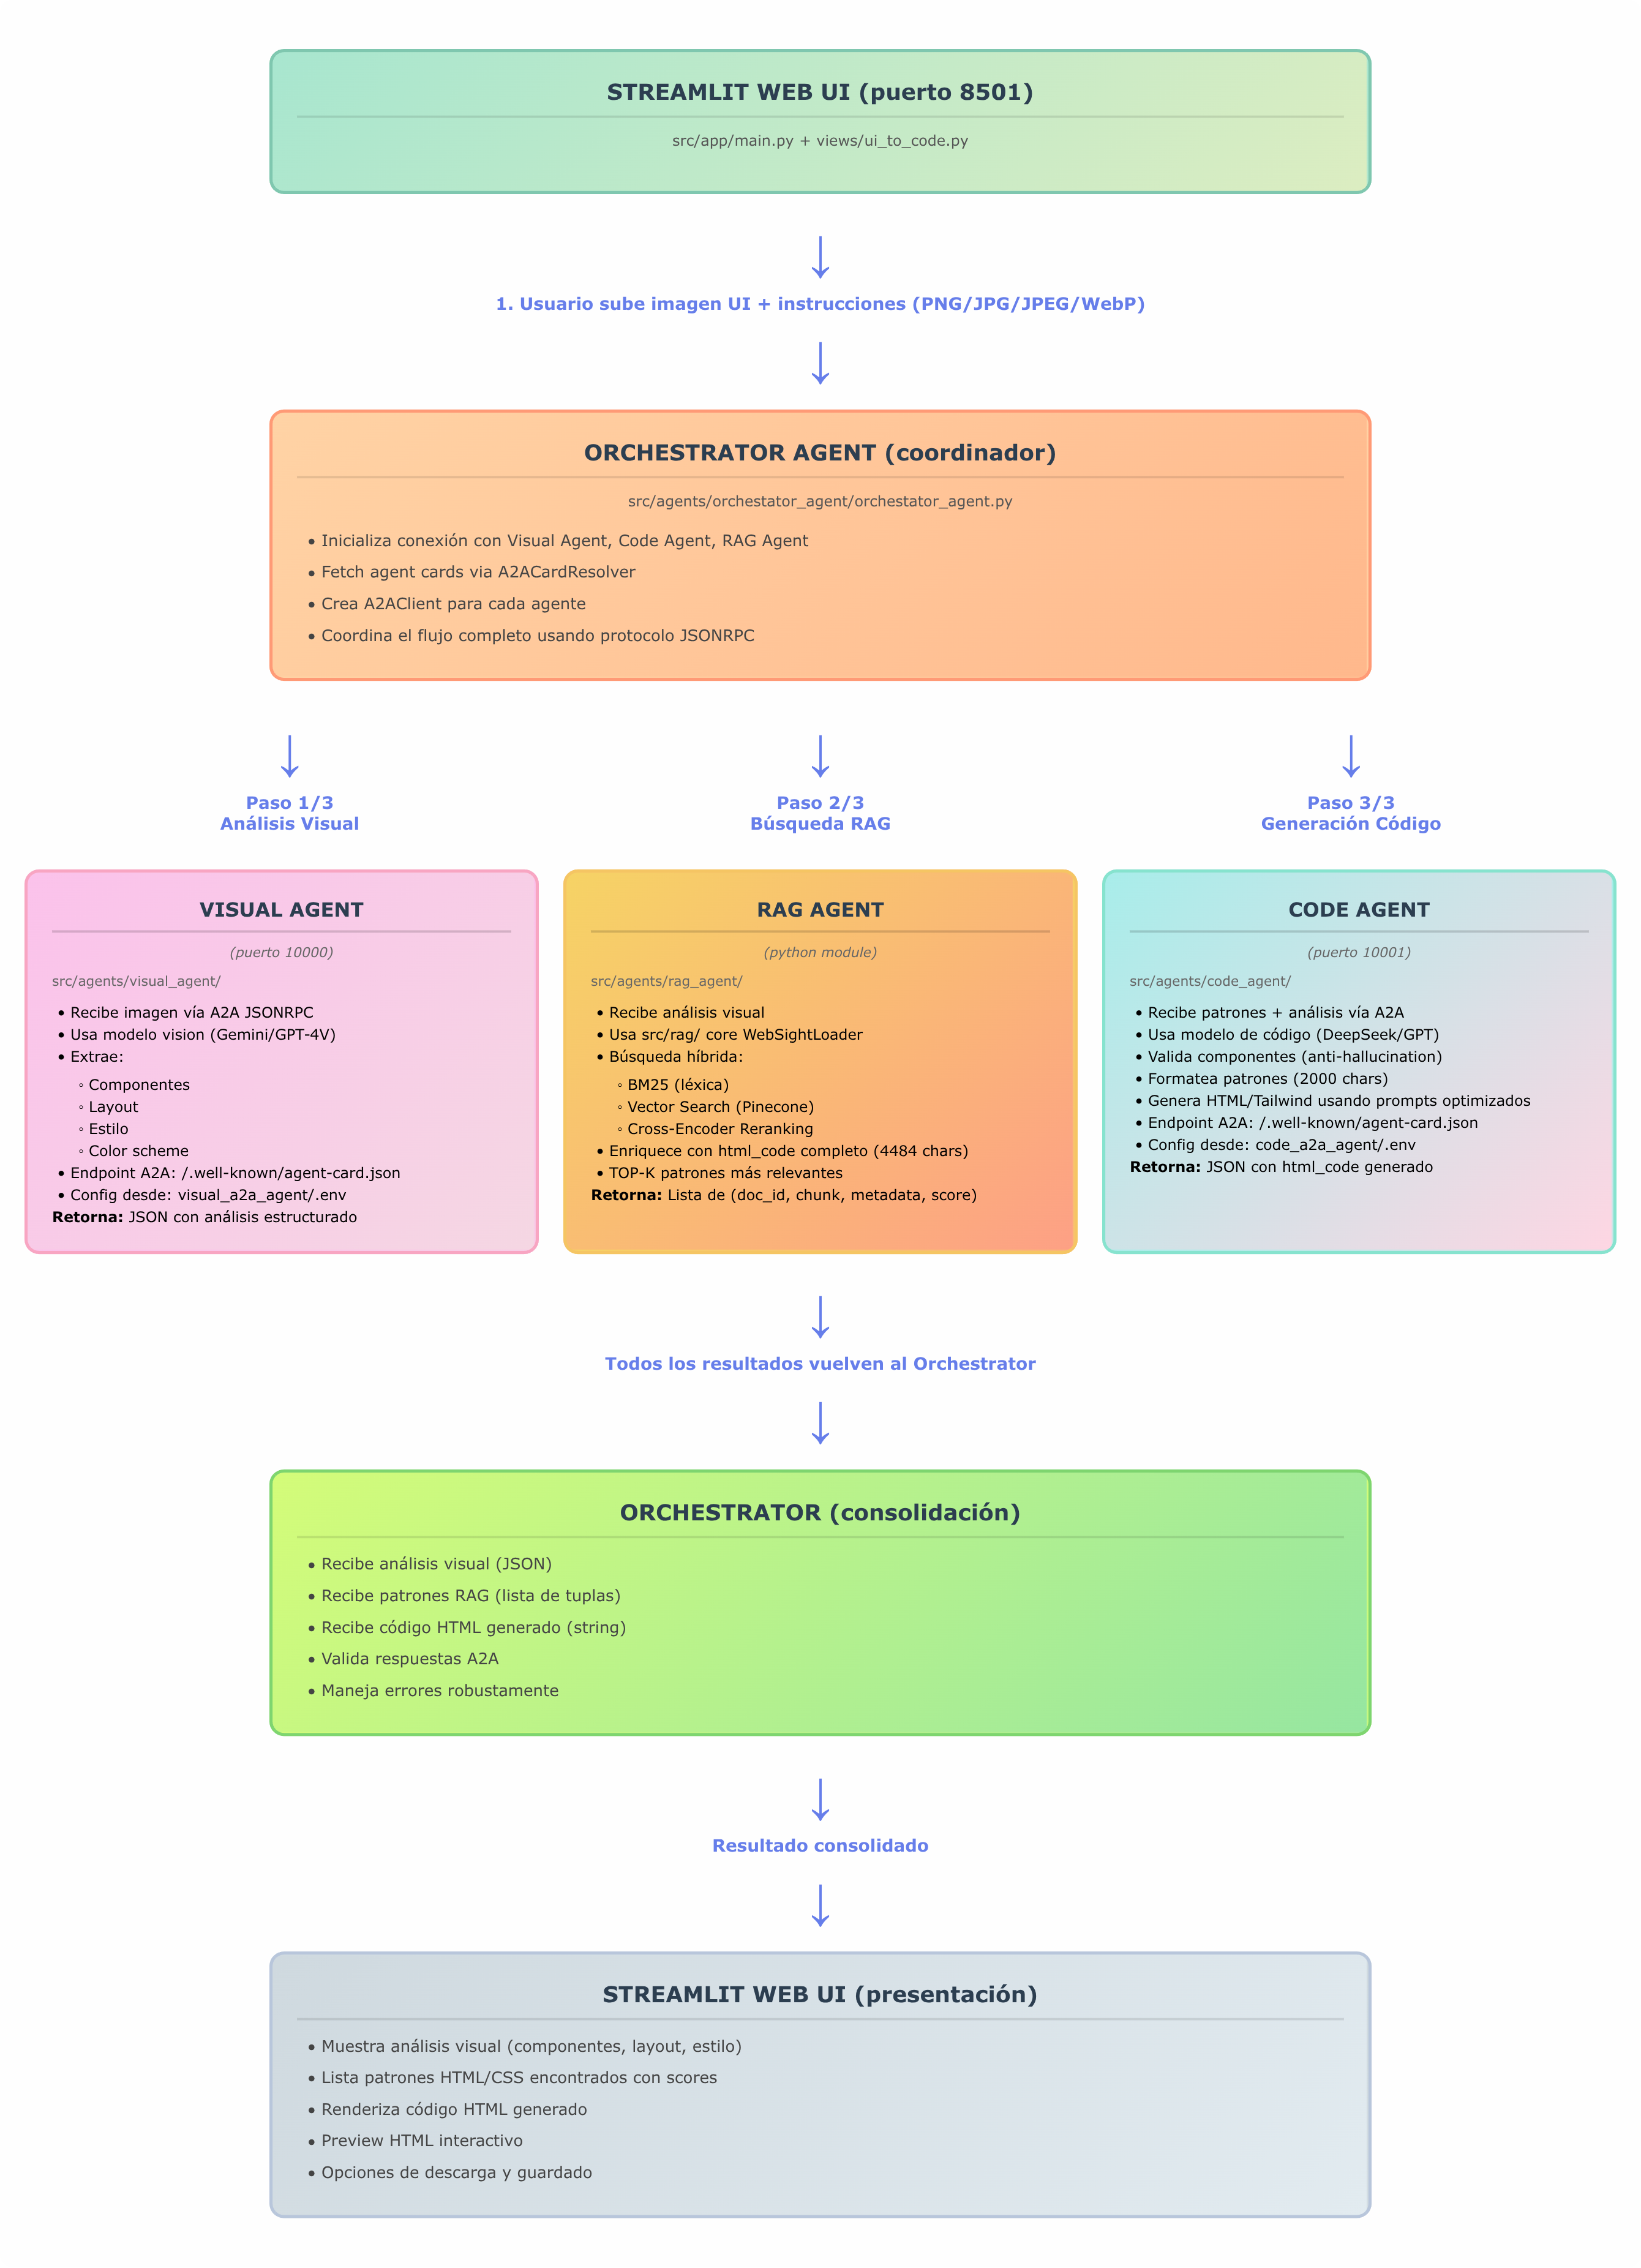
\includegraphics[width=\textwidth]{../docs/diagrama-flujo-arquitectura-multi-agente.png}
\caption{Arquitectura Multi-Agente UI2Code}
\label{fig:arquitectura}
\end{figure}

\begin{enumerate}
    \item Usuario sube imagen UI + instrucciones en Streamlit (puerto 8501)
    \item Orchestrator Agent coordina la ejecución secuencial:
    \begin{itemize}
        \item \textbf{Paso 1/3}: Visual Agent analiza imagen vía A2A JSONRPC
        \item \textbf{Paso 2/3}: RAG Agent busca patrones similares
        \item \textbf{Paso 3/3}: Code Agent genera HTML usando análisis + patrones
    \end{itemize}
    \item Orchestrator consolida resultados y retorna a Streamlit
    \item Streamlit presenta: análisis visual, patrones encontrados, código generado, preview HTML
\end{enumerate}

\subsection{Pipeline RAG Detallado}

El sistema RAG implementa un flujo de tres fases como se muestra en la Figura \ref{fig:rag}:

\begin{figure}[H]
\centering
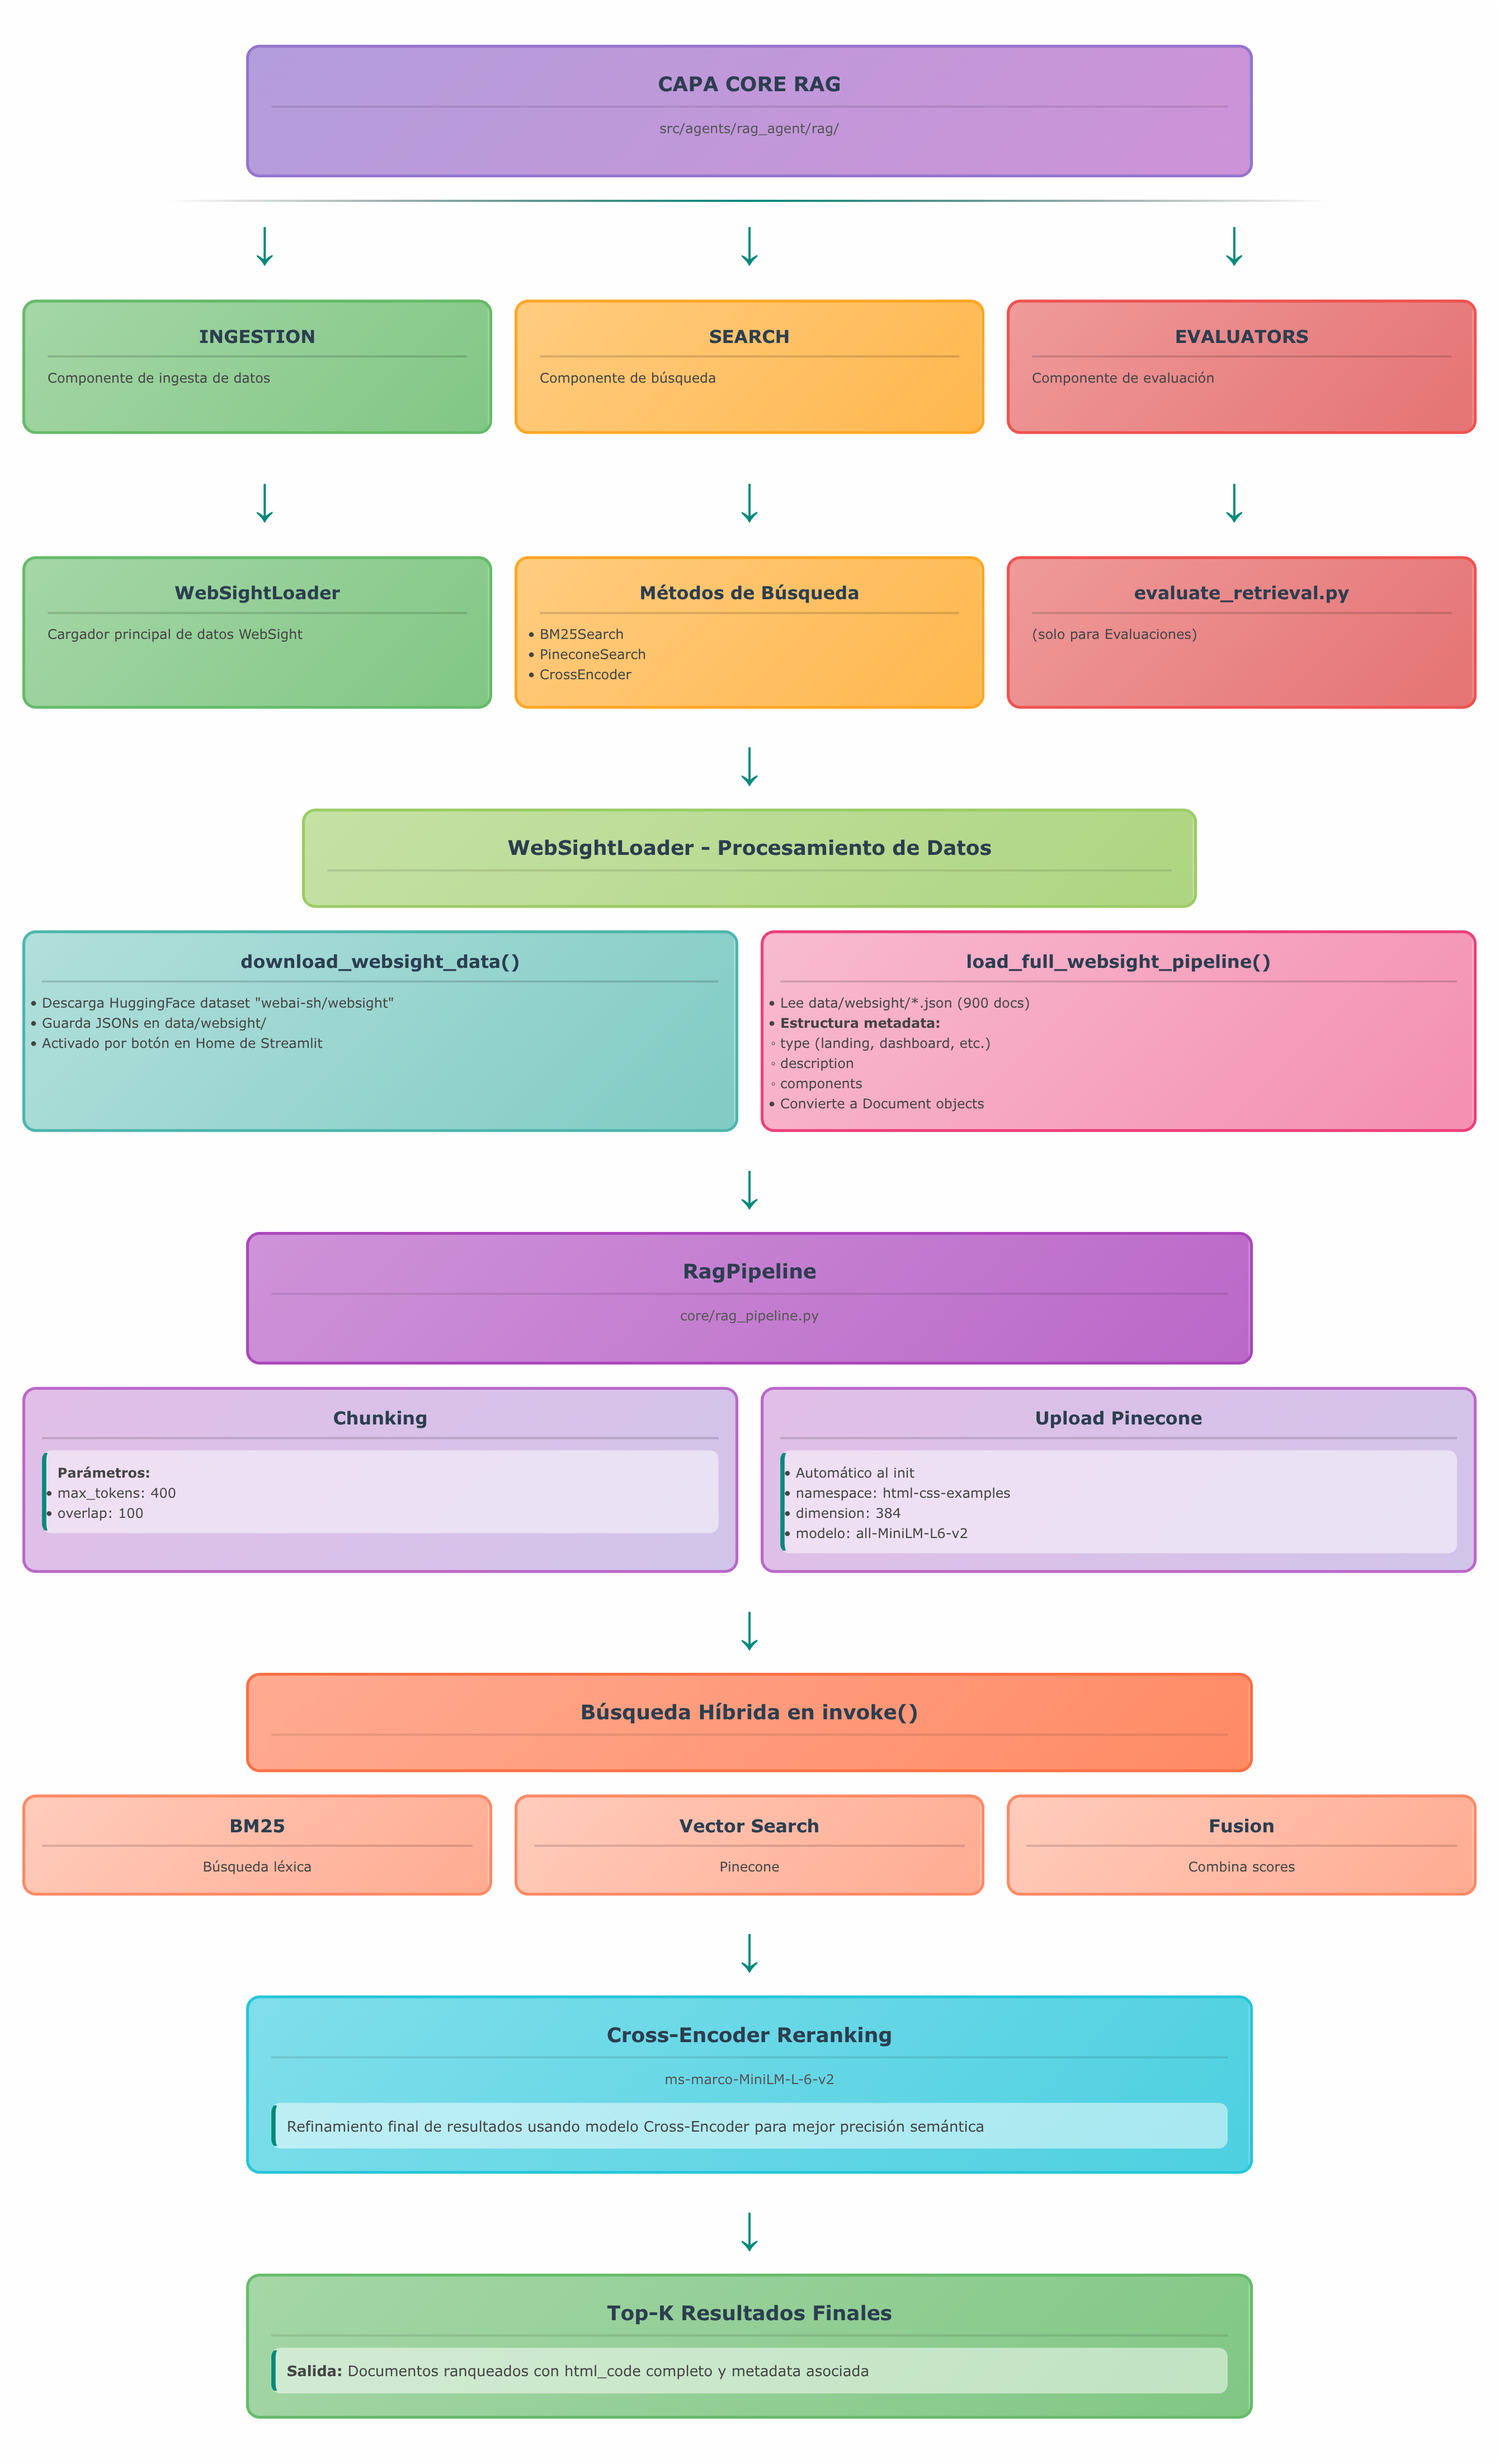
\includegraphics[width=0.9\textwidth]{../docs/diagrama-flujo-rag-pipeline.png}
\caption{Pipeline RAG Híbrido}
\label{fig:rag}
\end{figure}

\subsubsection{Fase 1: Ingesta de Documentos}
\begin{itemize}
    \item \texttt{WebSightLoader.download\_websight\_data()}: Descarga dataset desde HuggingFace
    \item Almacenamiento en \texttt{data/websight/*.json}
    \item \texttt{load\_full\_websight\_pipeline()}: Carga 900 documentos con metadata estructurado
    \item Conversión a objetos \texttt{Document} con campos: type, description, components
\end{itemize}

\subsubsection{Fase 2: Procesamiento}
\begin{itemize}
    \item \textbf{Chunking}: max\_tokens=400, overlap=100
    \item \textbf{Embedding}: \texttt{all-MiniLM-L6-v2} (384 dimensiones)
    \item \textbf{Upload a Pinecone}: Namespace \texttt{html-css-examples}
    \item Proceso automático al inicializar \texttt{RagPipeline}
\end{itemize}

\subsubsection{Fase 3: Búsqueda Híbrida (método \texttt{invoke()})}
\begin{enumerate}
    \item \textbf{BM25 Search}: Recuperación léxica de candidatos
    \item \textbf{Vector Search}: Consulta en Pinecone (cosine similarity)
    \item \textbf{Fusion}: Combina scores de ambos métodos con pesos configurables
    \item \textbf{Cross-Encoder Re-ranking}: Ordena candidatos por relevancia real
    \item \textbf{Enriquecimiento}: Agrega \texttt{html\_code} completo a metadata (hasta 4484 chars)
    \item \textbf{Top-k final}: Retorna los k resultados más relevantes
\end{enumerate}

\subsection{Protocolos de Comunicación}

\begin{table}[H]
\centering
\caption{Protocolos de Comunicación entre Componentes}
\begin{tabular}{ll}
\toprule
\textbf{Comunicación} & \textbf{Protocolo} \\
\midrule
Streamlit $\leftrightarrow$ Orchestrator & Python directo (\texttt{asyncio}) \\
Orchestrator $\leftrightarrow$ Visual Agent & A2A JSONRPC / HTTP (puerto 10000) \\
Orchestrator $\leftrightarrow$ Code Agent & A2A JSONRPC / HTTP (puerto 10001) \\
Orchestrator $\leftrightarrow$ RAG Agent & Python directo (módulo local) \\
RAG Agent $\leftrightarrow$ Pinecone & gRPC (Pinecone API) \\
\bottomrule
\end{tabular}
\end{table}

\subsection{Estructura de Directorios}

La estructura del proyecto está organizada modularmente:

\begin{lstlisting}[language=bash,caption={Estructura de Directorios Principal}]
ui2code-rag/
  |-- data/                        # Datos del sistema
  |     |-- evaluate/                # Framework de evaluacion
  |     |     |-- docs_ui_code_en.jsonl
  |     |     |-- qrels_ui_code_en.csv
  |     |     `-- eval_retrieval_*.csv
  |     |-- generated_code/          # HTML generados
  |     |-- temp_images/             # Imagenes temporales
  |     `-- websight/                # 900 JSONs corpus
  |-- docs/                        # Documentacion y diagramas
  |     |-- diagrama-flujo-arquitectura-multi-agente.png
  |     `-- diagrama-flujo-rag-pipeline.png
  |-- logs/                        # Logs del sistema
  |-- src/
  |     |-- agents/
  |     |     |-- code_a2a_agent/      # Code Agent (puerto 10001)
  |     |     |-- orchestator_agent/   # Coordinador
  |     |     |-- rag_agent/           # RAG + WebSight
  |     |     `-- visual_a2a_agent/    # Visual Agent (puerto 10000)
  |     |-- app/                     # Streamlit (puerto 8501)
  |     |     |-- main.py
  |     |     |-- pages/               # Paginas multipagina
  |     |     `-- views/               # Logica de vistas
  |     `-- common/                  # Utilidades comunes
  |-- docker-compose.yaml
  |-- Dockerfile
  |-- Makefile
  |-- run.sh                       # Script de inicio automatico
  `-- requirements.txt
\end{lstlisting}

\section{Flujo Funcional - Interfaz de Usuario}

El sistema expone una aplicación web Streamlit multipágina accesible en \texttt{http://localhost:8501} con cinco secciones principales.

\subsection{Página: Home}

\textbf{Funcionalidad}: Dashboard principal con estado del sistema.

\textbf{Características}:
\begin{itemize}
    \item Inicialización automática del corpus HTML/CSS (900 documentos WebSight)
    \item Botón de descarga del dataset si \texttt{data/websight/} está vacío
    \item Proceso: \texttt{ensure\_rag\_ready()} $\rightarrow$ \texttt{WebSightLoader.download\_websight\_data()}
    \item Navegación rápida a todas las funcionalidades
    \item Métricas del sistema: agentes activos, documentos cargados, índice Pinecone
\end{itemize}

\subsection{Página: UI to Code (Principal)}

\textbf{Funcionalidad}: Conversión de imágenes de diseños UI a código HTML/Tailwind CSS.

\textbf{Flujo de uso}:
\begin{enumerate}
    \item \textbf{Upload de imagen}: Drag \& drop o selección de archivo (PNG/JPG/JPEG/WebP)
    \item \textbf{Instrucciones personalizadas} (opcional, bilingüe español/inglés):
    \begin{itemize}
        \item Estilo: ``Usar tema oscuro con acentos púrpura''
        \item Responsive: ``Hacer completamente responsive con diseño mobile-first''
        \item Interactividad: ``Agregar efectos hover sutiles y animaciones''
        \item Accesibilidad: ``Incluir etiquetas ARIA y alto contraste''
    \end{itemize}
    \item \textbf{Ejecución}: Click en ``Generar código''
    \item \textbf{Visualización de resultados}:
    \begin{itemize}
        \item Análisis visual (componentes, layout, estilo, paleta)
        \item Patrones HTML/CSS encontrados (expandibles con scores)
        \item Código HTML generado (editor con syntax highlighting)
        \item Preview HTML interactivo (iframe)
    \end{itemize}
    \item \textbf{Descarga}: Guardado automático en \texttt{data/generated\_code/}
\end{enumerate}

\textbf{Procesamiento interno}:
\begin{enumerate}
    \item Orchestrator envía imagen a Visual Agent vía A2A
    \item Visual Agent retorna análisis estructurado JSON
    \item RAG Agent ejecuta búsqueda híbrida sobre corpus
    \item Code Agent genera HTML usando análisis + patrones + instrucciones
    \item Validación anti-hallucination con \texttt{\_validate\_html\_components()}
    \item Consolidación y presentación de resultados
\end{enumerate}

\subsection{Página: Query Interface}

\textbf{Funcionalidad}: Búsqueda de patrones HTML/CSS usando RAG + generación desde prompt.

\textbf{Modos de operación}:
\begin{itemize}
    \item \textbf{Modo búsqueda}: Recupera patrones similares del corpus
    \item \textbf{Modo Prompt$\rightarrow$HTML}: Genera código desde descripción textual
\end{itemize}

\textbf{Parámetros configurables}:
\begin{itemize}
    \item \texttt{top\_k}: Número de resultados a mostrar (1-20)
    \item \texttt{top\_retrieve}: Candidatos antes de re-ranking (5-200)
    \item \texttt{use\_reranking}: Activar/desactivar Cross-Encoder
    \item \texttt{include\_summary}: Resúmenes generados por IA
\end{itemize}

\textbf{Visualización}:
\begin{itemize}
    \item Resultados clasificados con scores de relevancia
    \item Código fuente completo de cada patrón
    \item Metadata: tipo de documento, descripción, componentes
    \item Resumen contextual (si está habilitado)
\end{itemize}

\subsection{Página: Evaluaciones}

\textbf{Funcionalidad}: Framework de evaluación de rendimiento del sistema RAG.

\textbf{Dataset de evaluación}:
\begin{itemize}
    \item \texttt{data/evaluate/docs\_ui\_code\_en.jsonl}: 9 documentos HTML
    \item \texttt{data/evaluate/qrels\_ui\_code\_en.csv}: Labels de relevancia
\end{itemize}

\textbf{Configuración de evaluación}:
\begin{itemize}
    \item \texttt{k}: Valores para métricas (ej: 3, 5, 10)
    \item \texttt{top\_retrieve}: Candidatos a recuperar (5-200)
    \item \texttt{top\_final}: Resultados después de re-ranking (1-50)
    \item \texttt{device}: CPU/CUDA/MPS para procesamiento
\end{itemize}

\textbf{Métricas calculadas}:
\begin{itemize}
    \item \textbf{Precision@k}: Proporción de resultados relevantes en top-k
    \item \textbf{Recall@k}: Proporción de documentos relevantes recuperados
    \item \textbf{nDCG}: Normalized Discounted Cumulative Gain (calidad de ranking)
    \item \textbf{MRR}: Mean Reciprocal Rank (posición del primer relevante)
\end{itemize}

\textbf{Visualización}:
\begin{itemize}
    \item Tabla por query: métricas detalladas
    \item Tabla agregada: promedios macro por k
    \item Botones de descarga en CSV
    \item Comparación pre/post re-ranking
\end{itemize}

\subsection{Página: System Status}

\textbf{Funcionalidad}: Monitoreo en tiempo real del sistema.

\textbf{Información mostrada}:
\begin{itemize}
    \item \textbf{Estado de agentes}:
    \begin{itemize}
        \item Visual Agent (puerto 10000): Online/Offline
        \item Code Agent (puerto 10001): Online/Offline
        \item Verificación de endpoints A2A
    \end{itemize}
    \item \textbf{Métricas del corpus}:
    \begin{itemize}
        \item Total de documentos: 900 (WebSight)
        \item Total de chunks indexados
        \item Estado del índice Pinecone
    \end{itemize}
    \item \textbf{Configuración activa}:
    \begin{itemize}
        \item Modelos en uso (VISUAL\_MODEL, CODE\_MODEL)
        \item Parámetros de chunking
        \item Endpoints de agentes
    \end{itemize}
\end{itemize}

\subsection{Página: Corpus Information}

\textbf{Funcionalidad}: Exploración del corpus HTML/CSS.

\textbf{Características}:
\begin{itemize}
    \item \textbf{Navegación de documentos}:
    \begin{itemize}
        \item Lista de 900 documentos WebSight
        \item Filtrado por tipo (landing, dashboard, form, etc.)
    \end{itemize}
    \item \textbf{Vista previa}:
    \begin{itemize}
        \item Código HTML completo
        \item Metadata: description, components, type
    \end{itemize}
    \item \textbf{Estadísticas}:
    \begin{itemize}
        \item Distribución de tipos de documento
        \item Longitud promedio de documentos
        \item Estadísticas de fragmentación (chunks)
    \end{itemize}
\end{itemize}

\section{Gobernanza de Calidad y Anti-Alucinación}

\subsection{Estrategias Implementadas}

\subsubsection{RAG como Contexto Obligatorio}

Los prompts del Code Agent incluyen citas explícitas de patrones recuperados para ``anclar'' la generación:

\begin{itemize}
    \item Patrones formateados con primeros 2000 caracteres de HTML
    \item Referencias directas a estructura técnica de ejemplos
    \item Instrucciones para usar patrones como guía, no como copia literal
\end{itemize}

\subsubsection{Guardrails de Validación}

Sistema de validaciones en múltiples capas:

\begin{table}[H]
\centering
\caption{Guardrails Implementados}
\begin{tabular}{llp{5cm}}
\toprule
\textbf{Guardrail} & \textbf{Hub} & \textbf{Función} \\
\midrule
\texttt{valid\_json} & Sí & Verifica formato JSON válido (no schema) \\
\texttt{web\_sanitization} & Sí & Detecta y escapa caracteres sospechosos (librería \texttt{bleach}) \\
\texttt{valid\_schema\_json} & No & Valida schema Pydantic específico (custom del equipo) \\
\texttt{is\_html\_field} & No & Valida HTML con BeautifulSoup (custom del equipo) \\
\bottomrule
\end{tabular}
\end{table}

\subsubsection{Validación Anti-Hallucination en Code Agent}

Método \texttt{\_validate\_html\_components()} implementado en Code Agent:

\begin{itemize}
    \item \textbf{Detección}: Identifica secciones HTML extra (header, nav, footer, aside)
    \item \textbf{Comparación}: Contrasta con componentes del análisis visual
    \item \textbf{Logging}: Warnings detallados cuando hay discrepancias
    \item \textbf{Ejemplo}: Si el análisis visual pide ``login form'', pero el código genera ``landing page completa con header y footer'', el sistema logea una advertencia
\end{itemize}

\subsubsection{Prompts Optimizados con Reglas Críticas}

Extracto del prompt del Code Agent (\texttt{src/agents/code\_agent/src/texts/prompts.py}):

\begin{lstlisting}[language=Python,caption={Fragmento de Prompt Anti-Hallucination}]
CRITICAL RULES:
1. Generate ONLY components mentioned in visual analysis
2. DO NOT add header, nav, footer unless explicitly requested
3. Use patterns as technical reference, not literal base
4. If visual analysis says "login form", generate ONLY login form
5. DO NOT hallucinate complete landing pages from single components
\end{lstlisting}

\subsubsection{Fallback Controlado}

Cuando la evidencia visual es insuficiente:

\begin{itemize}
    \item Sistema detecta baja confianza en análisis (imagen borrosa, ambigua)
    \item En lugar de alucinar, comunica: \textit{``Evidencia insuficiente para generar código. Por favor, proporcione una imagen más nítida y especifique 2-3 componentes clave.''}
    \item Evita generación de código no utilizable
\end{itemize}

\subsubsection{Umbrales de Confianza en Recuperación}

\begin{itemize}
    \item Si el recall efectivo del RAG cae bajo umbral configurado
    \item Sistema solicita: mayor nitidez de imagen O instrucciones adicionales
    \item Previene generación con contexto pobre
\end{itemize}

\subsection{Hallazgos Clave}

\begin{enumerate}
    \item \textbf{Few-shots + patrones RAG reducen alucinación}: Restringir la libertad del LLM con ejemplos concretos y patrones recuperados disminuye significativamente la alucinación de layouts complejos.
    
    \item \textbf{Esquemas estrictos evitan salidas mal formadas}: Los schemas Pydantic/Guardrails previenen respuestas fuera de contrato, pero pueden introducir errores de validación si el LLM se desvía (ej: listas vacías, campos omitidos).
    
    \item \textbf{Nitidez de imagen es crítica}: La calidad visual de la imagen de entrada impacta directamente en la fidelidad del código generado.
    
    \item \textbf{Re-ranking estabiliza prompts largos}: El Cross-Encoder mejora la estabilidad del top-k y reduce el drift en prompts con mucho contexto.
    
    \item \textbf{Separación de agentes facilita debugging}: La arquitectura multi-agente permite prompts más simples por agente y debugging localizado.
\end{enumerate}

\section{Implementación y Tooling}

\subsection{Tecnologías Core}

\begin{table}[H]
\centering
\caption{Stack Tecnológico}
\begin{tabular}{lll}
\toprule
\textbf{Componente} & \textbf{Tecnología} & \textbf{Versión} \\
\midrule
Modelos IA & OpenRouter & API v1 \\
Embeddings & Sentence-Transformers & $\geq$ 5.1.1 \\
Vector DB & Pinecone & $\geq$ 3.0.0 \\
Web UI & Streamlit & $\geq$ 1.28.0 \\
A2A Protocol & a2a-sdk & $\geq$ 0.3.8 \\
Guardrails & guardrails-ai & $\geq$ 0.6.7 \\
Logging & loguru & $\geq$ 0.7.3 \\
ASGI Server & Uvicorn & $\geq$ 0.37.0 \\
\bottomrule
\end{tabular}
\end{table}

\subsection{OpenRouter Integration}

\textbf{Ventajas}:
\begin{itemize}
    \item Acceso unificado a múltiples proveedores (Google, Anthropic, DeepSeek, OpenAI)
    \item Modelos gratuitos disponibles (Gemini Flash, DeepSeek R1 Distill)
    \item Modelos premium bajo demanda
    \item Gestión automática de rate limits y fallbacks
\end{itemize}

\textbf{Modelos recomendados}:
\begin{lstlisting}[caption={Configuracion de Modelos en .env}]
# Modelos gratuitos (recomendados)
VISUAL_MODEL=google/gemini-2.0-flash-exp:free
CODE_MODEL=deepseek/deepseek-r1-distill-llama-70b:free

# Alternativas premium (mejor calidad)
# VISUAL_MODEL=anthropic/claude-3.5-sonnet
# CODE_MODEL=deepseek/deepseek-r1
\end{lstlisting}

\subsection{Pinecone Vector Database}

\textbf{Configuración}:
\begin{itemize}
    \item Index: \texttt{pln3-index}
    \item Namespace: \texttt{html-css-examples} (corpus), \texttt{eval-metrics} (evaluación)
    \item Dimensión: 384 (all-MiniLM-L6-v2)
    \item Métrica: Cosine similarity
\end{itemize}

\textbf{Proceso de indexación}:
\begin{enumerate}
    \item WebSightLoader carga 900 documentos
    \item Chunking con max\_tokens=400, overlap=100
    \item Generación de embeddings con Sentence-Transformers
    \item Upload automático a Pinecone (solo si no existe)
    \item Verificación de conectividad en System Status
\end{enumerate}

\subsection{Streamlit como UI Acelerada}

\textbf{Características utilizadas}:
\begin{itemize}
    \item Arquitectura multipágina con \texttt{st.Page}
    \item Componentes interactivos: \texttt{st.file\_uploader}, \texttt{st.text\_area}, \texttt{st.expander}
    \item Columnas responsivas con \texttt{st.columns}
    \item Session state para persistencia
    \item Tema custom (paleta violeta) en \texttt{.streamlit/config.toml}
\end{itemize}

\subsection{Uvicorn + Starlette + A2A}

\textbf{Agentes A2A}:
\begin{itemize}
    \item Visual Agent y Code Agent exponen endpoints JSONRPC
    \item Servidor ASGI con Uvicorn
    \item Comunicación asíncrona (aunque actualmente síncrona en ejecución)
    \item Agent cards en \texttt{/.well-known/agent-card.json}
\end{itemize}

\textbf{Ejemplo de comunicación A2A}:
\begin{lstlisting}[language=Python,caption={Llamada A2A desde Orchestrator}]
# Orchestrator envia mensaje a Visual Agent
response = await orchestrator.send_message_to_visual_agent(
    image_path="data/temp_images/upload_12345.jpg"
)

# Visual Agent procesa y retorna JSON
visual_analysis = response["result"]["analysis"]
# {"components": [...], "layout": "...", "style": "...", ...}
\end{lstlisting}

\subsection{Configuración Dinámica}

\textbf{pyprojroot + YAML}:
\begin{itemize}
    \item \texttt{src/config.py}: Resuelve rutas relativas portables
    \item \texttt{src/config.yaml}: URLs de agentes, timeouts, parámetros
    \item Variables de entorno con python-dotenv
\end{itemize}

\textbf{Ejemplo de configuración}:
\begin{lstlisting}[caption={config.yaml - Endpoints Agentes}]
agents:
  visual_agent:
    url: http://localhost:10000
    timeout: 60
  code_agent:
    url: http://localhost:10001
    timeout: 120
\end{lstlisting}

\subsection{Scripts de Evaluación}

\textbf{Ubicación}: \texttt{src/agents/rag\_agent/rag/evaluators/evaluate\_retrieval.py}

\textbf{Uso}:
\begin{lstlisting}[language=bash,caption={Ejecucion de Evaluacion}]
python -m src.agents.rag_agent.rag.evaluators.evaluate_retrieval \
  --docs data/evaluate/docs_ui_code_en.jsonl \
  --qrels data/evaluate/qrels_ui_code_en.csv \
  --ks 3,5 \
  --top_retrieve 10 \
  --top_final 5
\end{lstlisting}

\textbf{Salida}:
\begin{itemize}
    \item \texttt{eval\_retrieval\_per\_query.csv}: Métricas detalladas
    \item \texttt{eval\_retrieval\_aggregated.csv}: Promedios macro
\end{itemize}

\section{Organización del Proyecto y División del Trabajo}

\subsection{Distribución de Responsabilidades}

\begin{table}[H]
\centering
\caption{Matriz de Contribuciones del Equipo}
\begin{tabular}{lcccc}
\toprule
\textbf{Componente} & \textbf{Jorge} & \textbf{Bruno} & \textbf{Fabricio} & \textbf{Noelia} \\
\midrule
Estructura general del proyecto & D & D & C & C \\
Dockerización de la solución & C & D & C & D \\
Modelo de visión por computadora & D & D & D & D \\
Modelo de generación de código & D & C & C & C \\
Sistema de logging (loguru) & C & C & D & C \\
Arquitectura A2A & C & D & C & C \\
Guardrails & C & C & D & D \\
Corpus y generación de RAG & D & C & D & C \\
Interfaz visual (Streamlit) & C & C & C & D \\
\midrule
\textbf{TOTAL} & D:4, C:5 & D:4, C:5 & D:4, C:5 & D:4, C:5 \\
\textbf{Horas insumidas} & 40 hs & 40 hs & 40 hs & 40 hs \\
\bottomrule
\end{tabular}
\end{table}

\textit{Leyenda: D = Desarrollo (responsabilidad principal), C = Colaboración (soporte y revisión)}

\subsection{Metodología de Trabajo}

\begin{itemize}
    \item \textbf{Gestión}: Sprints semanales con reuniones de sincronización
    \item \textbf{Control de versiones}: Git con feature branches
    \item \textbf{Revisión de código}: Pull requests con revisión cruzada
    \item \textbf{Comunicación}: Slack + reuniones virtuales
    \item \textbf{Documentación}: Markdown en repositorio + comentarios en código
\end{itemize}

\section{Resultados y Estado Actual}

\subsection{Casos Positivos}

\begin{itemize}
    \item \textbf{UIs con estructura clara}: El sistema genera HTML/Tailwind coherente con grid/flex correctos, spacings razonables y componentes bien definidos (cards, buttons, forms).
    
    \item \textbf{Fallback seguro}: Ante imágenes borrosas o ambiguas, el sistema comunica proactivamente: \textit{``Evidencia insuficiente para generar código. Proporcione mejor nitidez y especifique 2-3 componentes clave.''}
    
    \item \textbf{RAG aporta consistencia}: Los snippets recuperados mejoran sustancialmente la consistencia estilística del código generado.
    
    \item \textbf{Código artesanal}: El HTML generado no depende de icon libraries externas, usando elementos geométricos simples y tipografía creativa.
    
    \item \textbf{Personalización bilingüe}: Las instrucciones en español o inglés funcionan correctamente para customizar el output.
\end{itemize}

\subsection{Limitaciones Observadas}

\begin{enumerate}
    \item \textbf{Estados de UI no reseteados}: En ciertos flujos, botones o controles quedaban deshabilitados por estados no correctamente reinicializados en Streamlit.
    
    \item \textbf{Validación de schemas}: El Code Agent puede fallar si el modelo genera listas vacías u omite campos esperados (ej: \texttt{components=[]}), cortando la interacción.
    
    \item \textbf{Excepciones en orquestación A2A}: Se observaron excepciones de \texttt{nest-asyncio} cuando respuestas parciales no respetan el contrato JSONRPC.
    
    \item \textbf{Layout en Query Interface}: El output de búsqueda aparecía en columna lateral en lugar de debajo del textarea (ajuste de layout en Streamlit).
    
    \item \textbf{Modelos gratuitos con limitaciones}: Los modelos free de OpenRouter tienen rate limits que pueden causar delays en desarrollo intensivo.
\end{enumerate}

\subsection{Resultados de Evaluación del Sistema RAG}

\begin{table}[H]
\centering
\caption{Métricas de Evaluación para Diferentes Valores de k}
\label{tab:metricas}
\begingroup
\footnotesize                 % achica fuente (podés probar \scriptsize)
\setlength{\tabcolsep}{4pt}   % menos espacio entre columnas (default ~6pt)
\begin{adjustbox}{max width=\linewidth}
\begin{tabular}{@{}ccccccccc@{}}
\toprule
\textbf{k} & \textbf{P@k Pre} & \textbf{R@k Pre} & \textbf{nDCG Pre} & \textbf{P@k Post} & \textbf{R@k Post} & \textbf{nDCG Post} & \textbf{MRR Pre} & \textbf{MRR Post} \\
\midrule
3 & 0.30 & 0.90 & 0.79 & 0.30 & 0.90 & 0.86 & 0.77 & 0.87 \\
5 & 0.20 & 1.00 & 0.83 & 0.20 & 1.00 & 0.90 & 0.77 & 0.87 \\
\bottomrule
\end{tabular}
\end{adjustbox}
\endgroup
\end{table}

\subsubsection{Significado de las Métricas}

\begin{itemize}
    \item \textbf{k}: Número de resultados considerados (top-k)
    \item \textbf{Precision@k (Pre/Post)}: Proporción de resultados relevantes en los primeros k (antes/después de re-ranking)
    \item \textbf{Recall@k (Pre/Post)}: Proporción de documentos relevantes recuperados en los primeros k
    \item \textbf{nDCG (Pre/Post)}: Normalized Discounted Cumulative Gain - calidad del ranking (mayor es mejor)
    \item \textbf{MRR (Pre/Post)}: Mean Reciprocal Rank - posición del primer resultado relevante (mayor es mejor)
\end{itemize}

\subsubsection{Interpretación de Resultados}

\begin{enumerate}
    \item \textbf{Alto recall (0.9 - 1.0)}: El sistema recupera casi todos los documentos relevantes en el top-k, indicando buena cobertura.
    
    \item \textbf{Precisión moderada (0.2 - 0.3)}: Hay presencia de resultados no relevantes en el top-k, sugiriendo espacio de mejora en filtrado.
    
    \item \textbf{Mejora por re-ranking}: El nDCG y MRR aumentan después del re-ranking (0.79$\rightarrow$0.86 y 0.77$\rightarrow$0.87), demostrando que el Cross-Encoder posiciona mejor los relevantes.
    
    \item \textbf{Recall no afectado por re-ranking}: Como esperado, el re-ranking no cambia qué documentos se recuperan, solo su orden.
    
    \item \textbf{Estabilidad en k=5}: Con k=5 se logra recall perfecto (1.0) manteniendo precisión razonable.
\end{enumerate}

\subsubsection{Resumen de Evaluación}

\begin{itemize}
    \item El sistema recupera casi todos los documentos relevantes (alto recall)
    \item La precisión podría mejorar con refinamiento de embeddings o ajuste de pesos BM25/Vector
    \item El re-ranking con Cross-Encoder mejora significativamente la posición de los relevantes
    \item Los resultados validan la efectividad del enfoque híbrido BM25 + Vector + Re-ranking
\end{itemize}

\section{Lecciones Aprendidas}

\begin{enumerate}
    \item \textbf{RAG + guardrails $>$ LLM puro}: Para la tarea de UI-to-Code, un sistema RAG con validaciones es significativamente superior a un LLM sin contexto.
    
    \item \textbf{Contratos de salida reducen alucinación}: Los schemas Pydantic/Guardrails fuerzan estructura, pero requieren diseño cuidadoso con campos opcionales y defaults para evitar rupturas de flujo.
    
    \item \textbf{Calidad de input es crítica}: Pedir al usuario 2-3 componentes clave y una imagen nítida mejora sustancialmente la fidelidad del código generado.
    
    \item \textbf{Re-ranking estabiliza prompts largos}: El Cross-Encoder reduce drift en prompts con mucho contexto, mejorando consistencia.
    
    \item \textbf{Separación de agentes facilita debugging}: La arquitectura multi-agente permite prompts más simples por componente y debugging localizado, aunque introduce complejidad de orquestación.
    
    \item \textbf{Docker simplifica despliegue}: La contenerización resolvió problemas de reproducibilidad entre entornos de desarrollo.
    
    \item \textbf{Modelos gratuitos son viables}: OpenRouter con modelos free (Gemini Flash, DeepSeek) permite MVP funcional, aunque con limitaciones de rate limits.
    
    \item \textbf{Logging estructurado es esencial}: Loguru facilitó debugging de flujos complejos multi-agente.
\end{enumerate}

\section{Roadmap Propuesto}

\subsection{Corto Plazo (1-3 meses)}

\subsubsection{Mitigación de Alucinación y UX}

\begin{itemize}
    \item Prompts con ``chain-of-thought estructurada'' no-verbatim para que Visual Agent reporte evidencias explícitas (colores, jerarquías, distancias relativas)
    \item Refuerzo con few-shots curados de HTML/Tailwind y contra-ejemplos (qué NO hacer)
    \item Validación incremental: primero estructura mínima (layout), luego detalles (estilos), evitando all-or-nothing del schema final
    \item Mejoras de UI: mover resultados siempre debajo del textarea, spinners por paso, mensajes de error accionables
\end{itemize}

\subsubsection{RAG y Corpus}

\begin{itemize}
    \item Aumentar corpus HTML/CSS a 2000+ documentos con ejemplos etiquetados por componentes y layouts (dashboard, e-commerce, forms)
    \item Embeddings específicos para código (e.g., code-aware models como CodeBERT)
    \item Re-ranking por coverage de componentes solicitados
    \item Persistir metadatos (tokens, longitud, nivel de nesting) para re-ranking semántico más fino
\end{itemize}

\subsection{Mediano Plazo (3-6 meses)}

\subsubsection{Agentes y Orquestación}

\begin{itemize}
    \item Retries con backoff exponencial y degradación graciosa cuando LLM viola contrato
    \item Relleno automático de campos faltantes en respuestas parciales
    \item Mensajería asincrónica real con tasks para cada generación (aprovechar A2A async)
    \item Implementación de MCP (Model Context Protocol) con tooling para RAG Agent
    \item LLM como orquestador dinámico en lugar de orquestador determinista
    \item Mejorar capa de persistencia (actualmente todo en memoria)
    \item Tests de contratos (Pydantic) per-commit con golden outputs
\end{itemize}

\subsubsection{Evaluación y Calidad}

\begin{itemize}
    \item Definir conjunto de imágenes canónicas con métricas de fidelidad:
    \begin{itemize}
        \item Component coverage score
        \item Layout IoU simplificado
        \item Developer acceptance testing
    \end{itemize}
    \item Automatizar batería de regresión con capturas y hashes de HTML resultante
    \item Tests robustos (actualmente solo MVP sin coverage completo)
\end{itemize}

\subsubsection{Costos y Observabilidad}

\begin{itemize}
    \item Estimación y tracking de costos por invocación
    \item Conteo de tokens utilizados con alertas de uso
    \item Telemetría con OpenTelemetry para observabilidad distribuida
    \item Dashboard de métricas de negocio (tiempo de generación, tasa de éxito, etc.)
\end{itemize}

\subsection{Largo Plazo (6+ meses)}

\begin{itemize}
    \item Fine-tuning de modelos propios para Visual y Code Agents
    \item Integración con IDEs (VSCode extension)
    \item Soporte para frameworks adicionales (React, Vue, Angular)
    \item Sistema de feedback loop para mejora continua del corpus
    \item Multi-tenancy para empresas con estilos diferentes
\end{itemize}

\section{Desafíos Afrontados Durante el Trabajo}

\subsection{Elección de Modelos}

\textbf{Problema}: Por restricción presupuestaria, los miembros del equipo no contaban con acceso a modelos pagos de forma continua.

\textbf{Solución}:
\begin{itemize}
    \item Optar por modelos gratuitos de OpenRouter (Gemini Flash, DeepSeek R1 Distill)
    \item Enfrentar volatilidad: OpenRouter daba de baja modelos con frecuencia
    \item Estrategia de equipo: rotar entre diferentes modelos gratuitos, todos con resultados aceptables
    \item Implementar configuración flexible vía .env para cambiar modelos sin modificar código
\end{itemize}

\subsection{Ejecución en Pipeline de Procesos}

\textbf{Problema}: Al comienzo se usaba Makefile para levantar agentes, servers y artefactos del sistema. Esto era tedioso y requería múltiples terminales, haciendo lenta la etapa de desarrollo y QA.

\textbf{Solución}:
\begin{itemize}
    \item Dockerizar la solución completa con Docker Compose
    \item Crear script \texttt{run.sh} para automatizar configuración y despliegue
    \item Resultado: funcionamiento rápido y eficaz en todas las máquinas de desarrollo
    \item Beneficio adicional: portabilidad para despliegue en producción
\end{itemize}

\subsection{Gestión de Configuraciones}

\textbf{Problema}: Múltiples archivos .env (raíz, Visual Agent, Code Agent) causaban confusión sobre qué variables usar dónde.

\textbf{Solución}:
\begin{itemize}
    \item Script \texttt{run.sh} guía interactivamente la configuración
    \item Documentación clara en README sobre cada archivo .env
    \item Validación de configuraciones al inicio de cada agente
\end{itemize}

\subsection{Sincronización de Versiones de Librerías}

\textbf{Problema}: Conflictos de dependencias entre Streamlit, Guardrails y Sentence-Transformers.

\textbf{Solución}:
\begin{itemize}
    \item Usar \texttt{pyproject.toml} con Poetry/UV para resolución de dependencias
    \item Bloquear versiones críticas con constraints
    \item Separar dependencias de desarrollo y producción
\end{itemize}

\subsection{Performance de Evaluaciones}

\textbf{Problema}: Evaluaciones con 900 documentos y re-ranking eran lentas en CPUs locales.

\textbf{Solución}:
\begin{itemize}
    \item Parametrizar device (CPU/CUDA/MPS) en evaluaciones
    \item Cachear resultados de búsqueda vectorial
    \item Subconjunto de evaluación (9 docs) para pruebas rápidas
\end{itemize}

\section{Conclusiones}

El enfoque multi-agente combinado con RAG híbrido y guardrails ha demostrado ser efectivo para reducir alucinación y mejorar la utilidad del código HTML/Tailwind generado a partir de imágenes de interfaz de usuario.

\subsection{Logros Principales}

\begin{itemize}
    \item \textbf{Sistema funcional end-to-end}: UI operativa con flujo completo desde imagen hasta código descargable
    \item \textbf{RAG híbrido probado}: BM25 + Vector Search + Re-ranking con métricas validadas (Recall 0.9-1.0, nDCG mejora 7-9\%)
    \item \textbf{Arquitectura A2A robusta}: Comunicación JSONRPC entre agentes con fallbacks
    \item \textbf{Validaciones efectivas}: Guardrails custom y del Hub reducen alucinaciones
    \item \textbf{Tooling completo}: Evaluación, logging, monitoring, UI multipágina
    \item \textbf{Despliegue simplificado}: Docker Compose + script automático
\end{itemize}

\subsection{Desafíos Persistentes}

\begin{itemize}
    \item Validación robusta de schemas con tolerancia a errores
    \item Estado de UI y sincronización en Streamlit
    \item Operatoria asincrónica real entre agentes (actualmente síncrono)
    \item Limitaciones de modelos gratuitos (rate limits, disponibilidad)
\end{itemize}

\subsection{Valor del Proyecto}

El sistema ya ofrece una base funcional y extensible para:

\begin{itemize}
    \item Acelerar desarrollo frontend con código estandarizado
    \item Reducir deuda técnica mediante reutilización de patrones
    \item Servir como referencia de arquitectura multi-agente con RAG
    \item Facilitar investigación en mitigación de alucinaciones
\end{itemize}

Con el roadmap propuesto, el sistema puede evolucionar hacia mayor fidelidad visual, estabilidad operativa y medición reproducible de calidad, acercándose a un producto comercialmente viable.

\subsection{Próximos Pasos Inmediatos}

\begin{enumerate}
    \item Expandir corpus a 2000+ documentos
    \item Implementar validación incremental (layout $\rightarrow$ estilos)
    \item Añadir telemetría de costos y tokens
    \item Tests de regresión automatizados
    \item Documentar casos de uso con empresas piloto
\end{enumerate}

\section{Anexo - Setup y Operación}

\subsection{Requisitos Previos}

\subsubsection{Producción (Recomendado)}
\begin{itemize}
    \item Docker y Docker Compose instalados
    \item Puertos disponibles: 8501, 10000, 10001
    \item APIs keys:
    \begin{itemize}
        \item OpenRouter API Key (\url{https://openrouter.ai/settings/keys})
        \item Pinecone API Key (\url{https://pinecone.io/})
        \item Guardrails API Key (\url{https://hub.guardrailsai.com/keys})
    \end{itemize}
\end{itemize}

\subsubsection{Desarrollo}
\begin{itemize}
    \item Python 3.10 - 3.12
    \item pip o UV para gestión de paquetes
    \item Entorno virtual (venv o conda)
\end{itemize}

\subsection{Instalación y Ejecución - Producción}

\textbf{Paso 1}: Ejecutar script de configuración automática

\begin{lstlisting}[language=bash]
bash run.sh
\end{lstlisting}

\textbf{Paso 2}: El script realizará:
\begin{enumerate}
    \item Verificación de Docker y Docker Compose
    \item Solicitud interactiva de API keys
    \item Creación de archivos .env en ubicaciones correctas:
    \begin{itemize}
        \item \texttt{.env} (raíz): PINECONE\_API\_KEY
        \item \texttt{src/agents/visual\_a2a\_agent/.env}: OPENROUTER\_API\_KEY, VISUAL\_MODEL, GUARDRAILS\_API\_KEY
        \item \texttt{src/agents/code\_a2a\_agent/.env}: OPENROUTER\_API\_KEY, CODE\_MODEL, GUARDRAILS\_API\_KEY
    \end{itemize}
    \item Ejecución de \texttt{docker compose up --build}
\end{enumerate}

\textbf{Paso 3}: Acceder a la aplicación

\begin{itemize}
    \item URL: \url{http://localhost:8501}
    \item Página principal: UI to Code
\end{itemize}

\textbf{Nota}: La primera ejecución puede tardar $\sim$30 minutos descargando imágenes Docker ($\sim$30 GB).

\subsection{Instalación y Ejecución - Desarrollo}

\textbf{Paso 1}: Instalar dependencias

\begin{lstlisting}[language=bash]
# Crear entorno virtual
python -m venv venv
source venv/bin/activate  # Windows: venv\Scripts\activate

# Opcion 1: UV (mas rapido)
uv sync

# Opcion 2: Poetry
poetry install

# Opcion 3: pip
pip install -e .
\end{lstlisting}

\textbf{Paso 2}: Configurar variables de entorno

\begin{lstlisting}[language=bash]
# Copiar plantillas
cp .env.example .env
cp src/agents/visual_a2a_agent/.env.example \
   src/agents/visual_a2a_agent/.env
cp src/agents/code_a2a_agent/.env.example \
   src/agents/code_a2a_agent/.env

# Editar cada archivo .env con tus API keys
\end{lstlisting}

\textbf{Paso 3}: Configurar Guardrails

\begin{lstlisting}[language=bash]
# Configurar Guardrails
make run-guardrails-configuration

# O manualmente
guardrails configure
guardrails hub install hub://guardrails/regex_match
guardrails hub install hub://guardrails/valid_json
guardrails hub install hub://guardrails/web_sanitization
\end{lstlisting}

\textbf{Paso 4}: Iniciar agentes (3 terminales separadas)

\begin{lstlisting}[language=bash]
# Terminal 1: Visual Agent
make run-visual-agent

# Terminal 2: Code Agent
make run-code-agent

# Terminal 3: Streamlit
make run-server
\end{lstlisting}

\textbf{Paso 5}: Acceder a \url{http://localhost:8501}

\subsection{Comandos Make Disponibles}

\begin{lstlisting}[language=bash]
# Descargar dataset WebSight
make download-websight

# Configurar Guardrails
make run-guardrails-configuration

# Iniciar agentes
make run-visual-agent    # Puerto 10000
make run-code-agent      # Puerto 10001
make run-server          # Puerto 8501

# Evaluacion de retrieval
make evaluate-retrieval
\end{lstlisting}

\subsection{Guardrails - Descripción Técnica}

Guardrails UI es una interfaz para supervisar, gestionar y controlar aplicaciones impulsadas por IA, especialmente modelos de lenguaje. Proporciona un entorno visual donde los desarrolladores pueden definir reglas, límites y flujos de trabajo, asegurando que las respuestas cumplan con criterios de seguridad, precisión y consistencia.

Guardrail Hub es una plataforma centralizada para gestionar, compartir y reutilizar conjuntos de guardrails, facilitando el acceso a plantillas predefinidas y manteniendo consistencia en múltiples proyectos.
\newpage
\subsubsection{Guardrails Utilizados en el Proyecto}

\setlength\LTleft{0pt}
\setlength\LTright{0pt}

\begin{small} % o 
\setlength{\tabcolsep}{4pt} 
\begin{longtable}{@{}P{0.26\linewidth} P{0.12\linewidth} P{0.18\linewidth} P{0.44\linewidth}@{}}
\caption{Guardrails implementados} \\
\toprule
\textbf{Nombre} & \textbf{Hub} & \textbf{Agentes} & \textbf{Descripción} \\
\midrule
\endfirsthead

\multicolumn{4}{c}{\tablename\ \thetable\ -- Continuación} \\
\toprule
\textbf{Nombre} & \textbf{Hub} & \textbf{Agentes} & \textbf{Descripción} \\
\midrule
\endhead

\midrule
\multicolumn{4}{r}{Continúa en la siguiente página} \\
\endfoot

\bottomrule
\endlastfoot

ValidJson         & Sí & code, visual & Verifica formato JSON válido. No valida schema específico. \\
WebSanitization   & Sí & code         & Detecta y escapa caracteres sospechosos. Basado en la librería \texttt{bleach}. \\
ValidSchemaJson   & No & code, visual & Valida schema Pydantic predeterminado. Extensión de ValidJson creada por el equipo. \\
IsHTMLField       & No & code         & Verifica formato HTML válido. Basado en BeautifulSoup. Creado por el equipo. \\

\end{longtable}
\end{small}


\subsection{Sistema de Logging}

\textbf{Librería}: Loguru

\textbf{Características}:
\begin{itemize}
    \item Logs estructurados con colores
    \item Rotación automática por fecha
    \item Niveles configurables (DEBUG, INFO, WARNING, ERROR)
    \item Salida a consola y archivo
\end{itemize}

\textbf{Ubicación de logs}:
\begin{itemize}
    \item Desarrollo: consola del terminal
    \item Producción: \texttt{logs/ui2code.YYYY-MM-DD.log}
    \item Docker: logs del contenedor (accesibles con \texttt{docker logs})
\end{itemize}

\textbf{Información logueada}:
\begin{itemize}
    \item Respuestas completas de modelos
    \item Errores de validación de guardrails
    \item Warnings de anti-hallucination
    \item Tiempos de ejecución de cada agente
    \item Métricas de búsqueda RAG (scores, latencias)
\end{itemize}

\subsection{Dataset WebSight - Detalles Técnicos}

\textbf{Fuente}: HuggingFace (\texttt{HuggingFaceM4/WebSight})

\begin{table}[H]
\centering
\caption{Características del Dataset WebSight}
\begin{tabular}{lp{10cm}}
\toprule
\textbf{Campo} & \textbf{Descripción} \\
\midrule
Nombre completo & WebSight (parte del proyecto HuggingFaceM4) \\
Modalidades & Imágenes, Texto \\
Formato & Parquet (convertido a JSON localmente) \\
Idioma & Inglés \\
Tamaño total & Versión v0.2: 1.92 millones de filas; v0.1: 823 mil filas \\
Split & Solo ``train'' (entrenamiento) \\
Longitud de texto & \texttt{text}: 344-6,310 caracteres; \texttt{llm\_generated\_idea}: 25-566 caracteres \\
Licencia & Creative Commons BY 4.0 (cc-by-4.0) \\
\bottomrule
\end{tabular}
\end{table}

\textbf{Campos utilizados}:

\begin{itemize}
    \item \textbf{text}: Contiene código HTML completo. Se usa para:
    \begin{itemize}
        \item Crear archivos .html en \texttt{data/websight/}
        \item Generar chunks (max\_tokens=400, overlap=100)
        \item Crear embeddings y subirlos a Pinecone
    \end{itemize}
    
    \item \textbf{llm\_generated\_idea}: Descripción textual del componente. Se usa en:
    \begin{itemize}
        \item Modo evaluación para verificar recuperación relevante
        \item Metadata de documentos para contexto semántico
    \end{itemize}
\end{itemize}

\textbf{Subconjunto utilizado}:

Si bien el dataset contiene casi 2 millones de registros, se decidió utilizar un subconjunto de \textbf{900 documentos} por:

\begin{itemize}
    \item Restricciones de la capa gratuita de Pinecone
    \item Evitar tiempos excesivos de descarga (dataset completo $>$ 50GB)
    \item Fines académicos del proyecto
    \item Balance entre cobertura y rendimiento
\end{itemize}

\textbf{Expansión futura}: Se espera ampliar a 2000+ documentos en versión comercial para mejorar cobertura de patrones.

\subsection{Troubleshooting}

\subsubsection{Si no ves 900 documentos en el corpus}

\begin{enumerate}
    \item Verifica que \texttt{data/websight/} contenga archivos JSON
    \item Si está vacío, ejecuta desde Home de Streamlit: ``Descargar dataset WebSight''
    \item O manualmente: \texttt{python src/scripts/download\_websight.py}
    \item Reinicia Streamlit - el corpus se carga automáticamente
\end{enumerate}

\subsubsection{Si los agentes no inician}

\begin{enumerate}
    \item Verifica archivos .env:
    \begin{itemize}
        \item \texttt{src/agents/visual\_a2a\_agent/.env} debe tener \texttt{OPENROUTER\_VISUAL\_MODEL}
        \item \texttt{src/agents/code\_a2a\_agent/.env} debe tener \texttt{OPENROUTER\_CODE\_MODEL}
        \item \texttt{.env} raíz debe tener \texttt{PINECONE\_API\_KEY}
    \end{itemize}
    \item Usa \texttt{bash run.sh} para configuración automática
    \item Verifica puertos 10000, 10001, 8501 disponibles
\end{enumerate}

\subsubsection{Si hay alucinaciones en código generado}

\begin{itemize}
    \item Revisa logs del Code Agent - debe mostrar warnings de validación
    \item Verifica que el análisis visual sea preciso
    \item Usa imagen más nítida y proporciona 2-3 componentes clave
    \item Considera modelos más potentes (DeepSeek R1 70B, Claude 3.5)
\end{itemize}

\subsubsection{Si Pinecone no funciona}

\begin{enumerate}
    \item Verifica \texttt{PINECONE\_API\_KEY} en \texttt{.env} raíz
    \item Confirma que el índice existe y acepta dimensión 384
    \item Namespaces usados: \texttt{html-css-examples} (corpus), \texttt{eval-metrics} (evaluación)
    \item Verifica conectividad en página ``System Status''
\end{enumerate}

\section{Referencias}

\begin{enumerate}
    \item HuggingFace M4. (2024). \textit{WebSight Dataset}. \url{https://huggingface.co/datasets/HuggingFaceM4/WebSight}
    
    \item Guardrails AI. (2024). \textit{Guardrails Hub Documentation}. \url{https://hub.guardrailsai.com/}
    
    \item Pinecone. (2024). \textit{Pinecone Vector Database Documentation}. \url{https://docs.pinecone.io/}
    
    \item OpenRouter. (2024). \textit{OpenRouter API Documentation}. \url{https://openrouter.ai/docs}
    
    \item Streamlit. (2024). \textit{Streamlit Documentation}. \url{https://docs.streamlit.io/}
    
    \item A2A Protocol. (2024). \textit{Agent-to-Agent Communication Protocol}. \url{https://github.com/a2a-protocol/a2a}
    
    \item Robertson, S., \& Zaragoza, H. (2009). \textit{The Probabilistic Relevance Framework: BM25 and Beyond}. Foundations and Trends in Information Retrieval, 3(4), 333-389.
    
    \item Reimers, N., \& Gurevych, I. (2019). \textit{Sentence-BERT: Sentence Embeddings using Siamese BERT-Networks}. EMNLP 2019.
\end{enumerate}

\end{document}